\chapter{Verwendete Technologien}
\label{Verwendete Technologien}

\section{Angular 2}
Es gibt unzählige Frameworks und Technologien für die Webentwicklung mit Java\-Script. Die weite Verbreitung von dem Platzhirsch \emph{AngularJS} kann beispielsweise durch die Anzahl an mit dem Tag "`angularjs"' versehenen Fragen auf \texttt{stackoverflow.com} belegt werden. Januar 2017 sind es 213 992 Fragen. Im Vergleich dazu sind 20 343 Fragen mit einem entsprechendem \emph{Ember.js} Tag versehen und bei dem immer beliebter werdenden Framework \emph{React.js} von \emph{Facebook} sind es immerhin 30 222 \cite{stackoverflow}.

Angular (oder auch AngularJS) ist ein seit 2009 von Google Inc. entwickeltes Framework und Open-Source-Projekt für Single-Page-Applicationen, d.h. Applikationen, die nur aus einer einzelnen HTML-Seite bestehen und deren Inhalte dynamisch nachgeladen werden. Die Sofwareentwicklung mit Angular wird im Gegensatz zu Softwareentwicklung mit reinem JavaScript deutlich vereinfacht, indem dem Entwickler Strukturen und Bibliotheken vorgegeben und Entscheidungen abgenommen werden. Mit dem Model-View-ViewModel unterstützt Angular bidirektionales Databinding.

Seit 2015 wird Angular 2 entwickelt und die zugrunde liegende Architektur von Angular wurde in diesem Zuge komplett überarbeitet. Angular 2 ist somit auch nicht mehr zu Angular 1 kompatibel. Der offensichtlichste Unterschied zu Angular 1 ist die Sprache in der Angular 2 geschrieben ist. Es wurde auf den Javascript Aufsatz TypeScript gesetzt. Dieser wurde von Microsoft entwickelt und erweitert JavaScript um die Möglichkeit objektorientiert und typsicher zu programmieren. TypeScript kann zu nativem JavaScript transpiliert werden.

Weiterhin ist Angular 2 Komponenten-orientiert. Das bedeutet, dass eine Applikation in beliebig viele kleine Komponenten aufgeteilt werden können, die durch gekapselte Logik und Wiederverwendbarkeit geprägt sind. Jede Komponente besteht aus einem Template in HTML, einer zugehörigen Klasse in Typescript und Sytlesheets in CSS oder mithilfe von CSS-Präprozessoren wie SASS oder LESS.

Eine \texttt{HelloWorld}-Komponente würde in Angular 2 folgendermaßen aussehen:
\begin{codebox}
\begin{lstlisting}[style=typescript]
import {Component} from '@angular/core';

@Component({
  selector: 'hello-world',
  template: '<p>Hello world!</p>',
  styles: ['p {color: red}']
})
export class HelloWorldComponent {
}
\end{lstlisting}
\end{codebox}

Template und Styles würden in einer Komponente eines echten Projekts der besseren Wartbarkeit halber noch in einzelne Dokumente ausgelagert werden.

Diese \texttt{HelloWorld}-Komponente könnte dann in einer Eltern-Komponente mit
\begin{codebox}
\begin{lstlisting}[language=HTML]
<hello-world></hello-world>
\end{lstlisting}
\end{codebox}
eingebunden werden.

\section{Cordova}
Um mit den Standard-Webtechnologien HTML5, CSS und JavaScript eine offline-fähige mobile App entwickeln zu können, bedarf es einer Technologie, um Webanwendungen in native, mobile Apps zu verpacken. Laut Shotts ermöglicht das Open-Source-Framework Cordova genau das \cite{shotts:phonegap}.

Die so entstehende native App besteht, wie in Abbildung \ref{fig:cordova} zu sehen, aus einem WebView-Element, also einem Browserfenster, das die vorher erwähnte Webanwendung im Vollbild anzeigt. Über das WebView-Element können, wie in einem herkömmlichen Browser, HTML- und CSS-Dateien dargestellt und JavaScript-Code ausgeführt werden. Das WebView greift auf den Standardbrowser des Betriebssystems zurück und erlaubt es dem Benutzer mit der App zu interagieren.

Cordova stellt darüber hinaus über eine JavaScript-Programmierschnittstelle Plug-Ins zur Verfügung, um auf die darunterliegende Plattform zuzugreifen. Diese Plug-Ins teilen sich in Core Plug-Ins und Drittanbieter Plug-Ins auf. Core Plug-Ins werden vom Cordova Team zur Verfügung gestellt und erlauben zum Beispiel den Zugriff auf die Kamera oder das Dateisystem des Gerätes. Die Funktionalität von Cordova kann durch selbst entwickelte oder Drittanbieter-Plug-Ins zusätzlich erweitert werden. Als mögliche Beispiele für Drittanbieter-Plug-Ins nennt Shotts einen Barcode Scanner oder ein Plug-In, um Inhalte über soziale Netzwerke zu teilen \cite{shotts:phonegap}.

\begin{figure}[htb]
\centering
\caption{Cordova Architektur \cite{cordova}}
\label{fig:cordova}
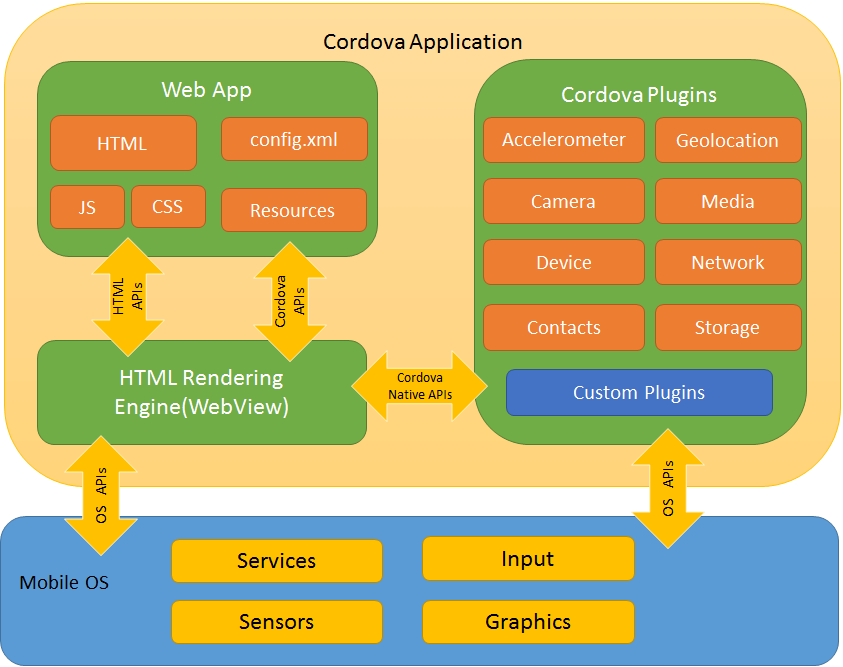
\includegraphics[width=0.8\textwidth]{\figdir/cordova.png}
\end{figure}

\section{Ionic}

Lässt sich Angular und Cordova miteinander verbinden, um die Vorteile von beiden Frameworks zu nutzen? Die Antwort ist ja. Das Open-Source-Framework Ionic bietet genau diese Verbindung zwischen Angular und Cordova. Hevery, der Schöpfer von Angular, beschreibt Ionic mit folgenden Worten:

\begin{citeenv}
	``Ionic is a shining example of a high-quality framework that takes advantage of Angular's power and flexibility, enabling developers to build production-ready mobile apps and Progressive Web Apps, in a fraction of the time.'' \cite{ionic:qutation}
\end{citeenv}


Mit Ionic kann eine Angular-Applikation sehr komfortabel plattformübergreifend in eine mobile Applikationen verwandelt werden. Es wird Ionic für Angular 1 und 2 angeboten.

Ionic bietet über die Funktionalität von Cordova hinaus fertige Angular-Komponenten an, die sich der Zielplattform entsprechend anpassen. Dadurch bekommt der Nutzer der mobilen Applikation das gewohnte Look-and-Feel des verwendeten Betriebssystems. Von Ionic werden die Plattformen iOS, Android und Windows Phone unterstützt. Es sind Komponenten wie \texttt{Header}, \texttt{Tabs} oder \texttt{List} verfügbar, die wie in Kapitel \ref{Verwendete Technologien} anhand der \texttt{HelloWorld}-Komponente veranschaulicht, im HTML-Template verwendet werden können. In Abbildung \ref{fig:loog-and-feel} wird am Beispiel von der Komponente \texttt{Action Sheet} das unterschiedliche Layout auf den unterstützten Plattformen illustriert.

\begin{figure}[htb]
\centering
\caption{Look-and-feel von Ionic auf verschiedenen Plattformen am Beispiel von Action Sheets}
\label{fig:loog-and-feel}
\begin{subfigure}{0.32\textwidth}
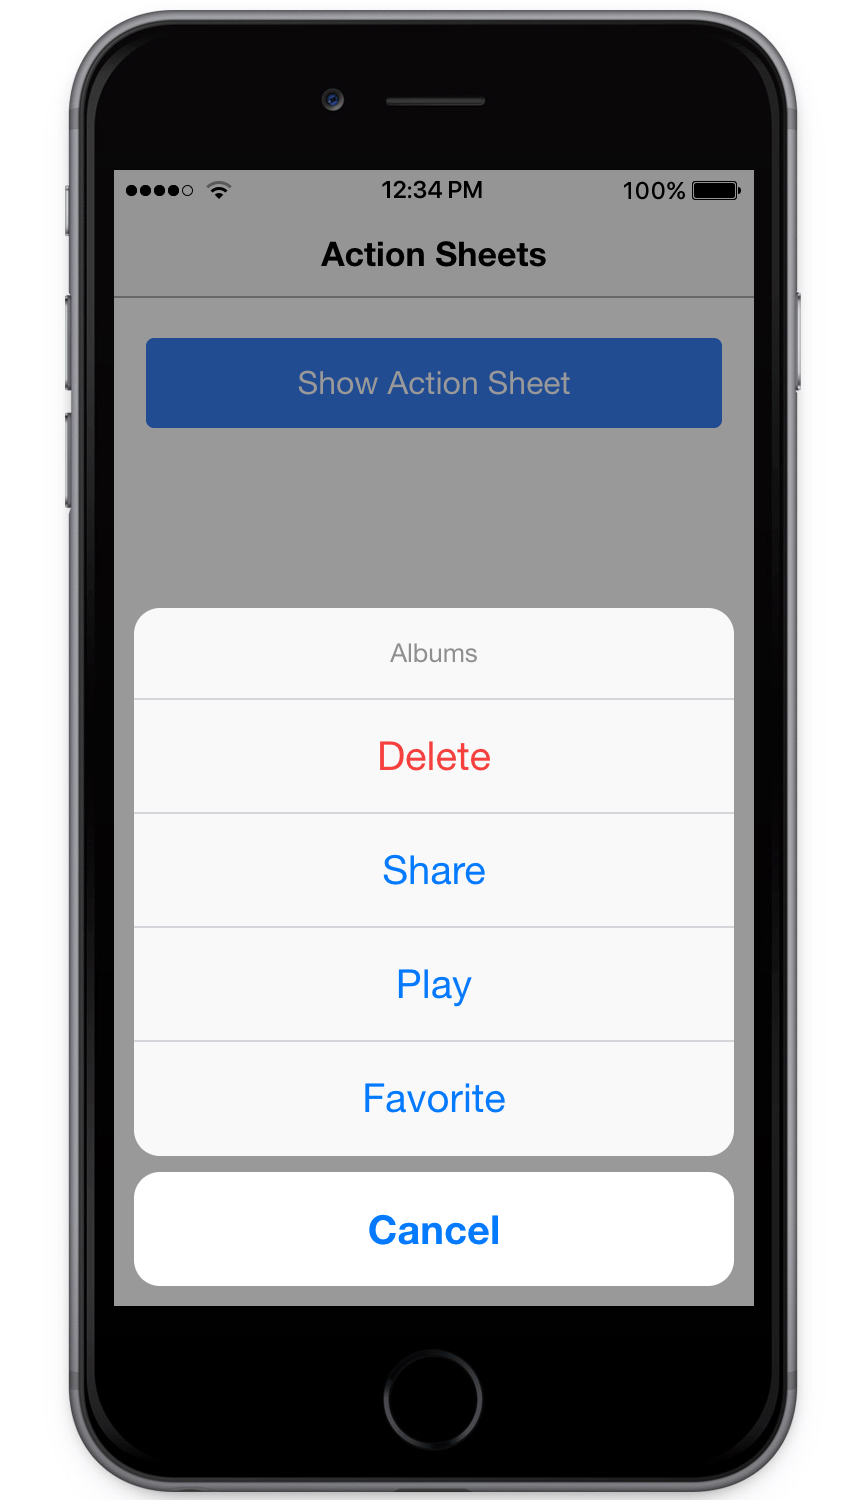
\includegraphics[width=\textwidth]{\figdir/ios}
\caption{iOS}
\end{subfigure}
\begin{subfigure}{0.32\textwidth}
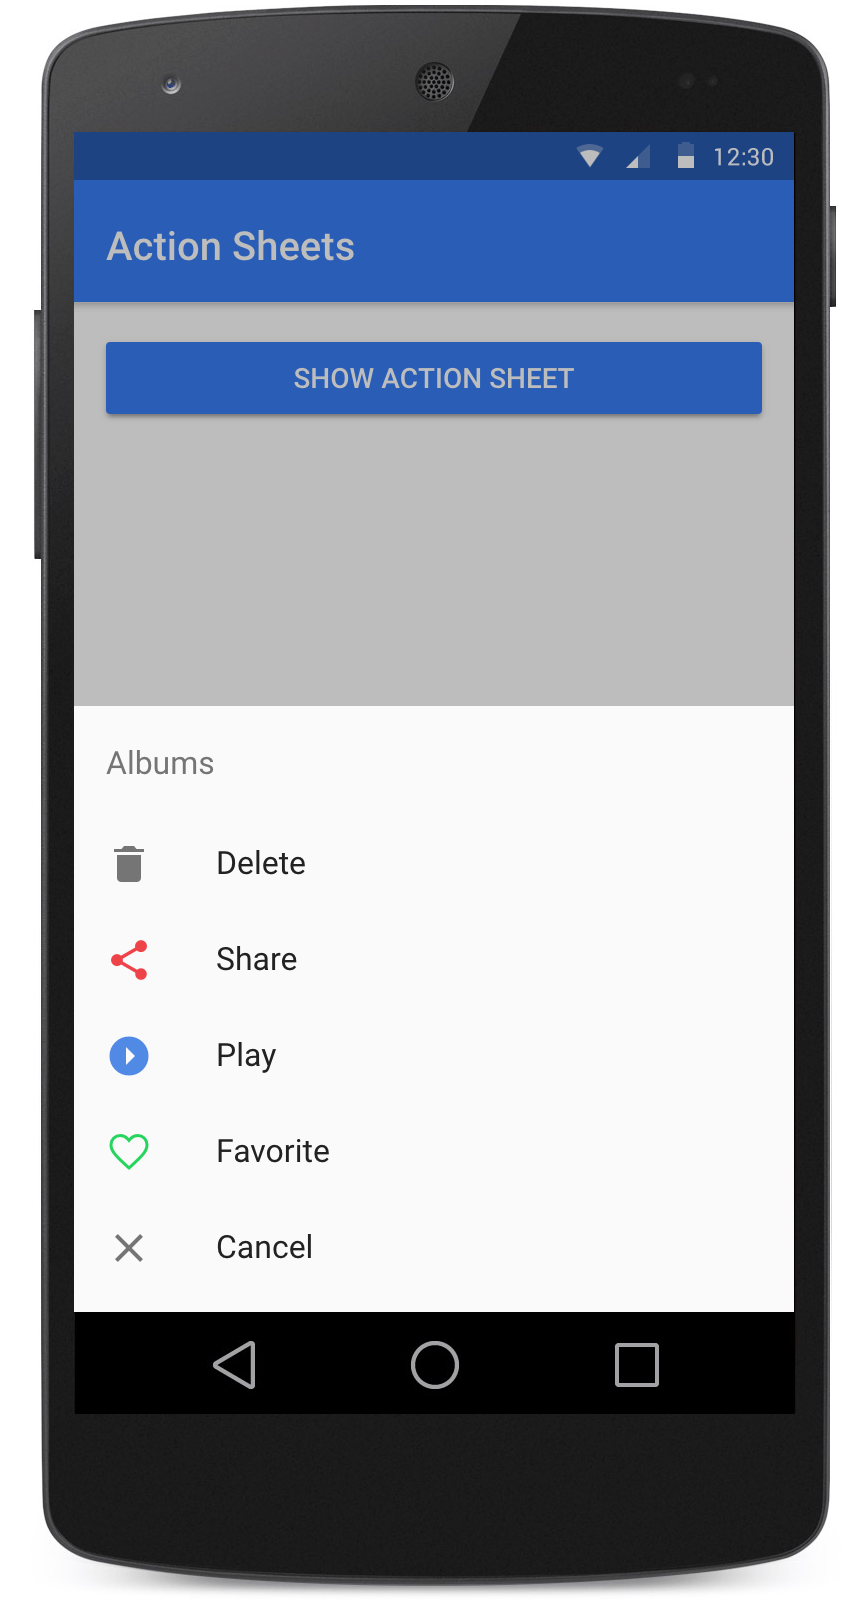
\includegraphics[height=8.4cm]{\figdir/android}
\caption{Android}
\end{subfigure}
\begin{subfigure}{0.32\textwidth}
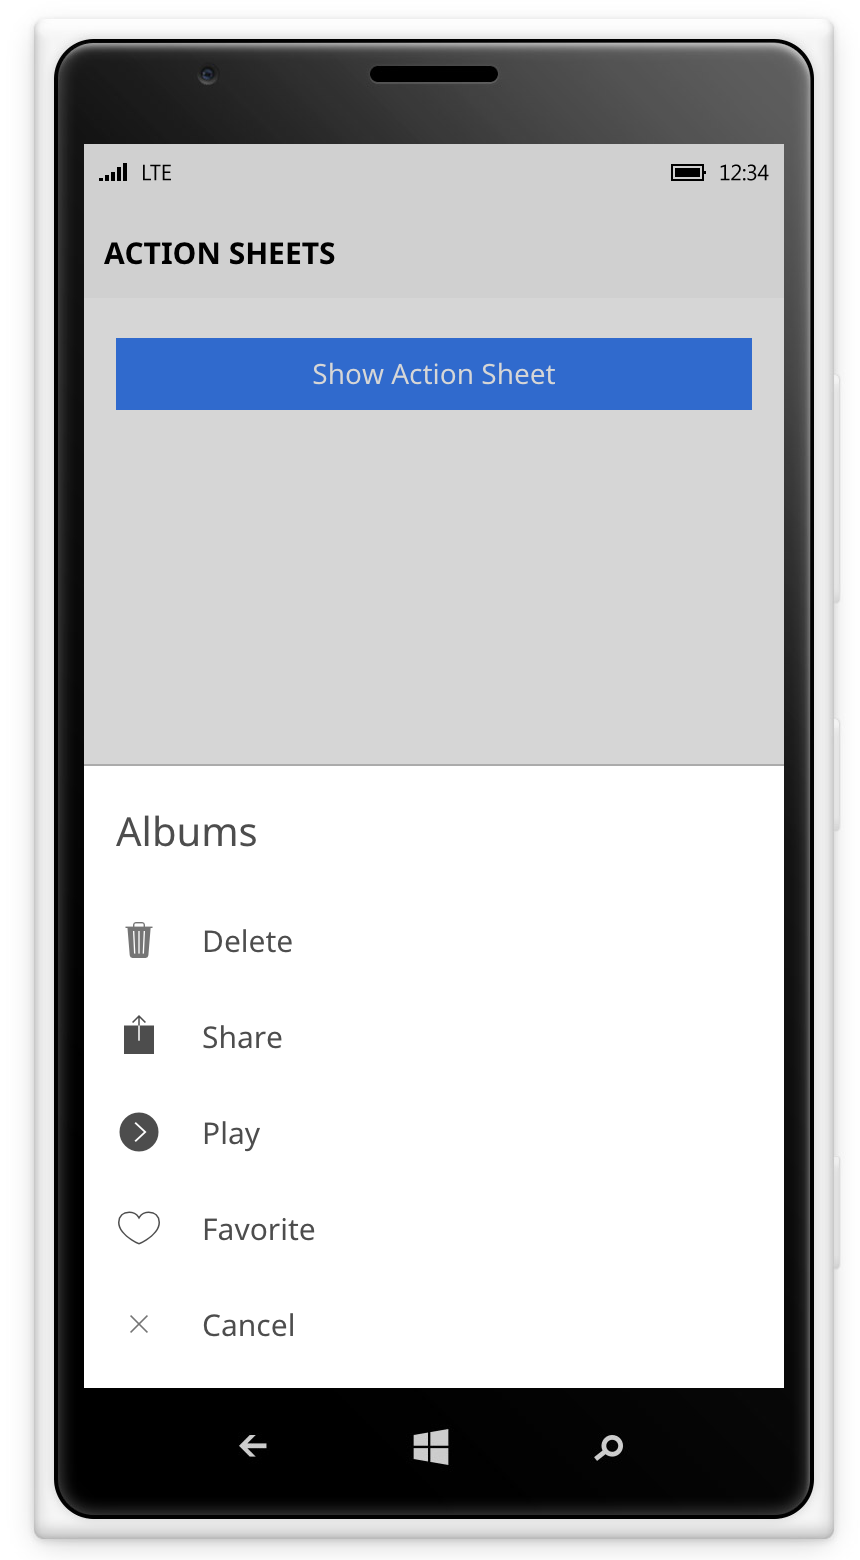
\includegraphics[width=\textwidth]{\figdir/wp}
\caption{Windows Phone}
\end{subfigure}
\end{figure}

Es wird deutlich, dass auch unterschiedliche Symbole verwendet werden. Dies passiert bei Verwendung von Ionic-Icons, von denen hunderte verfügbar sind, alles automatisch im Hintergrund.

Weiterhin können die Schnittstellen und Plugins von Cordova in TypeScript typsicher verwendet werden, sodass zum Beispiel per TypeScript auf die Kamera zugegriffen werden kann.

Insgesamt wurden bis Januar 2017 3,1 Millionen mobile Applikationen mit Ionic entwickelt. Auf den Entwicklungsprozess wird im nächsten Kapitel näher eingegangen.




